This is the reference manual for ProR.

\section{Editors}

Upon opening a ReqIF Model, the ReqIF Editor opens that provides an
overview of the model. A model contains any number of specifications,
and each specification is opened in its own editor.

\subsection{ReqIF Overview Editor}

\subsection{Specification Editor}

\section{Views}

By default, ProR shows three views.

\subsection{Project View}\index{Project View}

\subsection{Properties View}\index{Properties View}

\subsection{Outline View}\index{Outline View}

\section{Configurations}

The ProR menu contains entries to launch a number of configuration
dialogs.

\subsection{General Configuration}\index{Configuration!General}

\subsection{Datatype Configuration}\index{Configuration!Datatype}

This configuration is opened via ProR \textbar{} Datatype Configuration
...

The dialog shows two folders, one for SpecTypes and one for Datatypes.
SpecTypes are created for typing elements that have attributes
(SpecObjects, Specifications, SpecRelations). New SpecTypes can be
created by right-clicking on the folder and selecting ``New Child''.
Through the same mechanism, attribute definitions can be added to a
SpecType. attribute definitions are typed. Selecting an element shows
its properties in the lower pane, where it can be configured.

Attribute definitions must have a name and a datatype. Some attribute
definitions allow further customization. The datatype is selected from a
dropdown. New datatypes can be created by right-clicking on the folder
``Datatypes'' and selecting ``New Child''. Again, selecting a datatype
shows its properties in the lower pane, where it can be configured. A
datatype should have at least a long name.

As an example, consider the following Datatype Configuration Dialog:

\begin{figure}[h!]
\centering      
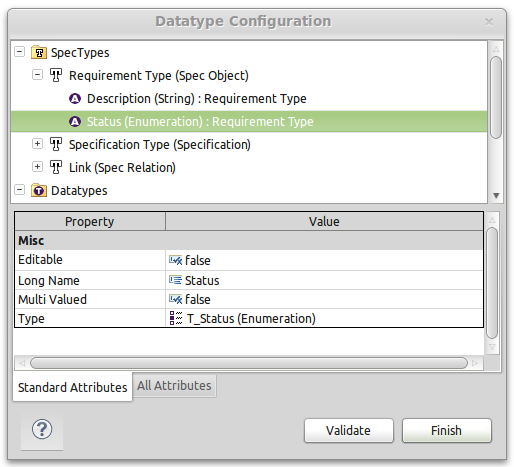
\includegraphics[width=0.8\linewidth]{../rmf-images/pror_datatype_configuration.png}
\caption{Datatype Configuration Dialog}      
\label{fig:DatatypeConfig}
\end{figure}

The Spec Type for ``Requirements Type'', which is applicable to
SpecObjects, is expanded. The Spec Type has two attributes,
``Description'' (String) and ``Status'' (Enumeration). Status is
selected, and in the pane below the mandatory values, ``Long Name'' and
``Type'' have been set. Further customization of the attribute is
possible, e.g. by converting it in a Multi-Valued attribute by setting
the corresponding flag to ``true''.

\subsubsection{Enumeration Datatypes}

An enumeration datatype must have enumeration values. These are created
by right-clicking the enumeration datatype and selecting New Child
\textbar{} Enum Value. You may have to unfold the enum value to select
it, so that you can provide it with a Long Name. The following shows a
correctly configured enumeration datatype:

\begin{figure}[h!]
\centering      
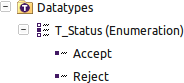
\includegraphics[width=0.4\linewidth]{../rmf-images/rmf_enumeration.png}
\caption{Enumerations}      
\label{fig:Enumerations}
\end{figure}

\subsection{Presentation Configuration}\index{Configuration!Presentation}

\subsection{Column Configuration}\index{Configuration!Column}

This configuration is specific to the Specification Editor.

The Column Configuration Dialog configures the Columns of a
Specification. Columns are identified by name. The width of the column
can be adjusted directly by dragging the column separator in the table
header.

If the SpecObject has an attribute where the name of the attribute
matches the name of the column, then that attribute is shown in that
column.
